\section{Introduzione}

Lo scopo di questa esperienza di laboratorio è quello di montare un impianto da vuoto che risulti in
grado di raggiungere pressioni dell'ordine di $10^{-3}$ \si{\pascal}. Inoltre l'esperienza serve anche a
prendere dimestichezza con le varie componenti che costituiscono l'impianto da vuoto.
Infine l'ultimo obbiettivo, ad impianto funzionante, è quello di tarare un vacuometro Pirani.

\section{Materiale utilizzato}

Il materiale messo a nostra disposizione è il seguente:

\begin{itemize}
	\item{una camera con un volume di $5930 \pm 10$ \si{\centi\metre}$^3$;}
	\item{una pompa rotativa con pressione di vuoto limite dell'ordine di qualche Pascal;}
	\item{una pompa ibrida turbomolecolare-molecular drag con relativa elettronica;}
	\item{cravatte e O-ring in Viton di varie dimensioni;}
	\item{tubi e raccordi con flange;}
	\item{2 valvole a membrana, 1 valvola a perdita calibrata, 1 valvola gate;}
	\item{2 vacuometri Pirani, 1 vacuometro a ionizzazione a catodo caldo e 1 vacuometo a ionizzazione a catodo freddo;}
	\item{cavi e lettore AGC per i quattro sensori sopracitati;}
\end{itemize}

\section{Esecuzione dell'esperienza}

\subsection{Montaggio dell'impianto da vuoto}

Per quanto riguarda il montaggio dell'impianto da vuoto abbiamo utilizzato il materiale sopraelencato
prestando attenzione che fossero rispettate le richieste dei tecnici di laboratorio;
ovvero che l'impianto soddisfacesse i seguenti requisiti:

\begin{itemize}
	\item{si doveva poter isolare la pompa turbomolecolare dal resto dell'impanto. In pratica si doveva realizzare un bypass dotato di valvola che collegava la pompa rotativa direttamente alla camera. In questo modo è stato possibile portare la camera a pressioni di qualche Pascal partendo da quella atmosferica. Quindi è stato creato un prevuoto che ha consentito di far funzionare la pompa turbomolecolare. Infatti questa tipologia di pompe può funzionare solo in regime molecolare;} %non mi piace ancora come è scritta...
    %WTF temperatura? % temperatura atmosferica senza spegnere la pompa turbomolecolare (che tra l'altro ci mette parecchi minuti a fermarsi);}
	\item{si doveva avere la possibilità di riportare la camera da vuoto alla pressione atmosferica senza spegnere
    la pompa turbomolecolare;}
    \item{si è prestata attenzione all'accensione e allo spegnimento del vacuometro a catodo caldo onde evitare
    di bruciare il filamento. Tale vacuometro opera ad di sotto dei $10^{-4}$ \si{\pascal};}
\end{itemize}

Uno schema dell'impianto è riportato in figura \ref{fig:schema}.

\subsection{Taratura dei vacuometri Pirani}

Per tarare il vacuometro Pirani, che misurava la pressione in camera, abbiamo portato la pressione oltre il limite inferiore
della sensibilità dello strumento, specificato nel manuale. Il manuale riporta un range massimo di funzionamento che va da $10^{-2}$ \si{\pascal} fino a $10^5$ \si{\pascal}, anche se l'intervallo in cui la precisione è buona è tra 0.1 \si{\pascal} e $10^4$ \si{\pascal}. Abbiamo quindi impostato il voltaggio in uscita al valore di 2 Volt lavorando su un potenziometro. Dopo aver isolato la pompa turbomolecolare dal resto dell'impianto abbiamo riportato la pressione della camera alla pressione atmosferica. A questo punto si è impostato il valore di output del sensore a 10 Volt, lavorando su un secondo potenziometro. Infine abbiamo riportato la pressione in camera a bassa pressione per controllare che il voltaggio al limite inferiore fosse ancora 2 Volt. Può succedere infatti che nella regolazione del secondo potenziometro il primo si stari.

\subsection{Qualche dato}

La pressione da noi raggiunta, come misurata con il vacuometro a catodo caldo, è di circa:

\begin{equation}
    P = 6.85 \cdot 10^{-4} \; \si{\pascal}
\end{equation}

\begin{figure}[b!]
    \centering
   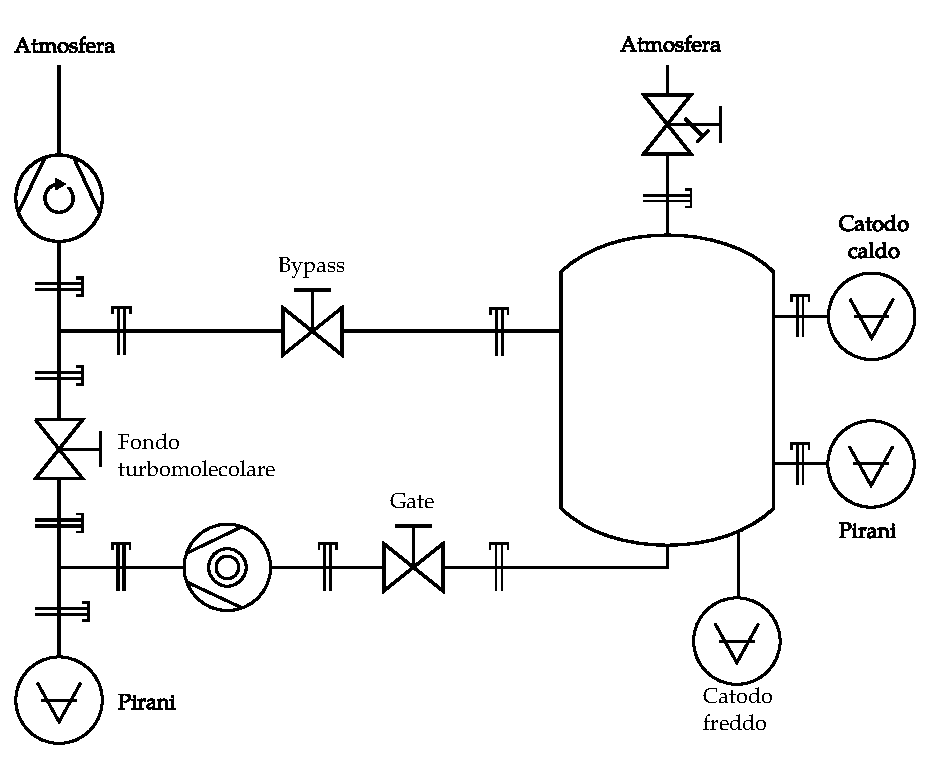
\includegraphics[width=16cm]{drawing.pdf}
   \caption{Schema dell'impianto da noi realizzato. La pompa primaria è una pompa rotativa, mentre la seconda pompa al centro dello schema
   è una pompa turbomolecolare. Sono visibili il bypass e i tre diversi sensori di pressione collegati alla camera da vuoto. La pompa
   turbomolecolare poteva essere isolata dal resto dell'impianto grazie alla valvola gate e alla valvola sul fondo della pompa.}
   \label{fig:schema}
\end{figure}

% direi che al grafico manca una legenda e dei riferimenti per capire cosa sono
% le cose attaccate al sistema. per indicare quali sono i vacuometri pirani/a catodo
% caldo/ a catodo freddo etc etc etc
